\documentclass[12pt]{article}


% The default font size is 10pt; 11pt and 12pt are alternatives
%%%%%%%%%%%%%%%%%%%%%%%%%%%%%%%%%%%%%%%%%
% Professional Newsletter Template
% Structural Definitions File
% Version 1.0 (09/03/14)
%
% Created by:
% Vel (vel@latextemplates.com)
%
% This file has been downloaded from:
% http://www.LaTeXTemplates.com
%
% License:
% CC BY-NC-SA 3.0 (http://creativecommons.org/licenses/by-nc-sa/3.0/)
%
%%%%%%%%%%%%%%%%%%%%%%%%%%%%%%%%%%%%%%%%%

%----------------------------------------------------------------------------------------
%	REQUIRED PACKAGES
%----------------------------------------------------------------------------------------

\usepackage{graphicx} % Required for including images
\usepackage{microtype} % Improved typography
\usepackage{multicol} % Used for the two-column layout of the document
\usepackage{booktabs} % Required for nice horizontal rules in tables
\usepackage{wrapfig} % Required for in-line images
\usepackage{float} % Required for forcing figures not to float with the [H] parameter
\usepackage{ragged2e} 

%encoding
%--------------------------------------
\usepackage[utf8]{inputenc}
\usepackage[T1]{fontenc}
%--------------------------------------

%French-specific commands
%--------------------------------------
\usepackage[french]{babel}
\usepackage[autolanguage]{numprint}

%------------------------------------------------
%Hyphenation rules
%--------------------------------------
\usepackage{hyphenat}
\hyphenation{mathéma-tiques récu-pérer}
%--------------------------------------

% Fonts

%-\usepackage{charter} % Use the Charter font as the main document font
%-\usepackage{courier} % Use the Courier font for \texttt (monospaced) only
%-\usepackage[T1]{fontenc} % Use T1 font encoding

%------------------------------------------------
% List Separation

%-\usepackage{enumitem} % Required to customize the list environments
%-\setlist{noitemsep,nolistsep} % Remove spacing before, after and within lists for a compact look

%------------------------------------------------
% Figure and Table Caption Styles

\usepackage{caption} % Required for changing caption styles
\captionsetup[table]{labelfont={bf,sf},labelsep=period,justification=justified} % Specify the table caption style
\captionsetup[figure]{labelfont={sf,bf},labelsep=period,justification=justified, font=small} % Specify the figure caption style
\setlength{\abovecaptionskip}{10pt} % Whitespace above captions

%------------------------------------------------
% Spacing Between Paragraphs

\makeatletter
\usepackage{parskip}
\setlength{\parskip}{6pt}
\newcommand{\@minipagerestore}{\setlength{\parskip}{6pt}}
\makeatother

%----------------------------------------------------------------------------------------
%	PAGE MARGINS AND SPACINGS
%----------------------------------------------------------------------------------------

\textwidth = 7 in % Text width
\textheight = 10 in % Text height
\oddsidemargin = -18pt % Left side margin on odd pages
\evensidemargin = -18pt % Left side margin on even pages
\topmargin = -36pt % Top margin
\headheight = 0pt % Remove the header by setting its space to 0
\headsep = 0pt % Remove the space between the header and top of the page
\parskip = 4pt % Space between paragraph
\parindent = 0.0in % Paragraph indentation
\pagestyle{empty} % Disable page numbering

%----------------------------------------------------------------------------------------
%	COLORS
%----------------------------------------------------------------------------------------

\usepackage[dvipsnames,svgnames]{xcolor} % Required to specify custom colors

\definecolor{altncolor}{rgb}{.8,0,0} % Dark red
%\definecolor{altncolor}{rgb}{.2,.4,.8} % Dark blue
%\definecolor{altncolor}{rgb}{.84,.16,.16} % Red

\usepackage[colorlinks=true, linkcolor=altncolor, anchorcolor=altncolor, citecolor=altncolor, filecolor=altncolor, menucolor=altncolor, urlcolor=altncolor]{hyperref} % Use the color defined above for all links

%----------------------------------------------------------------------------------------
%	BOX STYLES
%----------------------------------------------------------------------------------------

\usepackage[framemethod=TikZ]{mdframed}% Required for creating boxes
\mdfdefinestyle{sidebar}{
    linecolor=black, % Outer line color
    outerlinewidth=0.5pt, % Outer line width
    roundcorner=0pt, % Amount of corner rounding
    innertopmargin=10pt, % Top margin
    innerbottommargin=10pt, % Bottom margin
    innerrightmargin=10pt, % Right margin
    innerleftmargin=10pt, % Left margin
    backgroundcolor=white, % Box background color
    frametitlebackgroundcolor=white, % Title background color
    frametitlerule=false, % Title rule - true or false
    frametitlerulecolor=white, % Title rule color
    frametitlerulewidth=0.5pt, % Title rule width
    frametitlefont=\Large, % Title heading font specification
    font=\small
}

\mdfdefinestyle{intextbox}{
    linecolor=black, % Outer line color
    outerlinewidth=0.5pt, % Outer line width
    roundcorner=10pt, % Amount of corner rounding
    innertopmargin=7pt, % Top margin
    innerbottommargin=7pt, % Bottom margin
    innerrightmargin=7pt, % Right margin
    innerleftmargin=7pt, % Left margin
    backgroundcolor=white, % Box background color
    frametitlebackgroundcolor=white, % Title background color
    frametitlerule=false, % Title rule - true or false
    frametitlerulecolor=white, % Title rule color
    frametitlerulewidth=0.5pt, % Title rule width
    frametitlefont=\Large % Title heading font specification
}

%----------------------------------------------------------------------------------------
%	HEADING STYLE
%----------------------------------------------------------------------------------------

\newcommand{\heading}[2]{ % Define the \heading command
\vspace{#2} % White space above the heading
{\begin{center}\Large\textbf{#1}\end{center}} % The heading style
\vspace{#2} % White space below the heading
}

\newcommand{\BackToContents}{\hyperlink{contents}{{\small Back to Contents}}} % Define a command for linking back to the contents of the newsletter






%%% ---------------
%%% DEFINITIONS
%%% ---------------

% Define separators
\newcommand{\HorRule}[1]{\noindent\rule{\linewidth}{#1}} % Creating a horizontal rule
\newcommand{\SepRule}{\noindent							 % Creating a separator
						\begin{center}
							\rule{250pt}{1pt}
						\end{center}
						}

% Define Title en News input
\newcommand{\JournalName}[1]{%
		\begin{center}
			\Huge \usefont{T1}{QTCaligulatype}{m}{n}
			#1%
		\end{center}
		\par \normalsize \normalfont}

\newcommand{\JournalIssue}[1]{%
		\hfill \textsc{\mydate \today, No #1}
		\par \normalsize \normalfont}

\newcommand{\NewsItem}[1]{%
		\usefont{T1}{augie}{m}{n}
		\large #1 \vspace{4pt}
		\par \normalsize \normalfont}

\newcommand{\NewsAuthor}[1]{%
			\hfill by \textsc{#1} \vspace{4pt}
			\par \normalfont}
 % Include the document which specifies all packages and structural customizations for this template

\begin{document}


%----------------------------------------------------------------------------------------
%	HEADER IMAGE
%----------------------------------------------------------------------------------------

% Title
% -----
\JournalName{\Huge\textbf {GDPR FINES NEWSLETTER}}
\noindent\HorRule{3pt} \\[-0.75\baselineskip]
\HorRule{1pt}

\vspace{0.5cm}
	\SepRule
\vspace{0.5cm}


%General Statistic
\NewsItem{\raggedright{\LARGE GDPR Fines Overview}}
\justify
The General Data Protection Regulation 2016/679 is a regulation in EU law on data protection and privacy in the European Union and the European Economic Area. \\
\textbf{530} fines have been given out until today.
The overall cumulative total of data protection fines now stands at \textbf{275 187 314€}.


\begin{figure}
	[H]\centering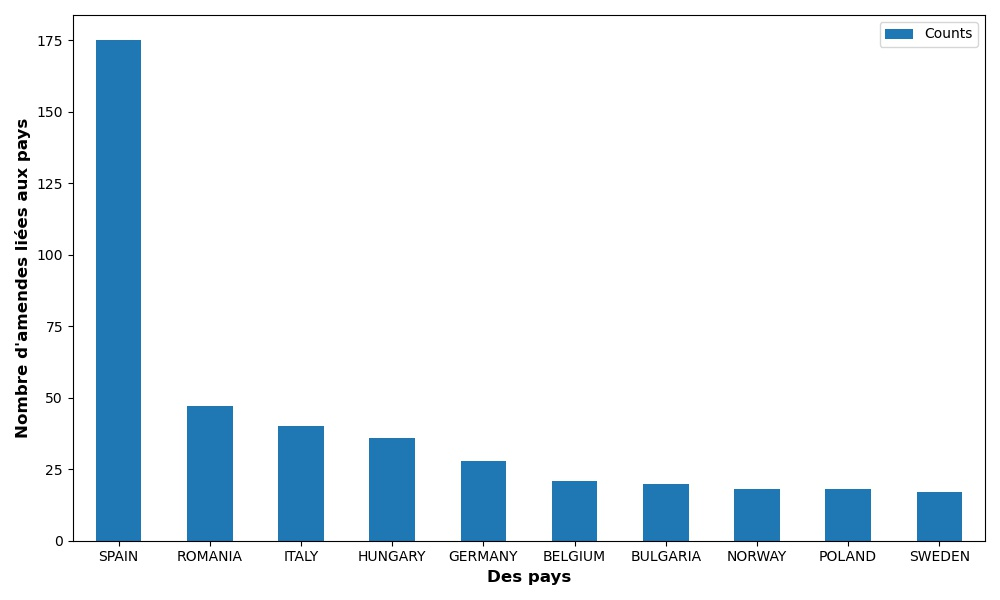
\includegraphics[width=0.7\linewidth]{graphs/top10_countries}
      \caption{Top 10 EU Countries with the highest number of fines }
\end{figure}
\begin{figure}
	[H]\centering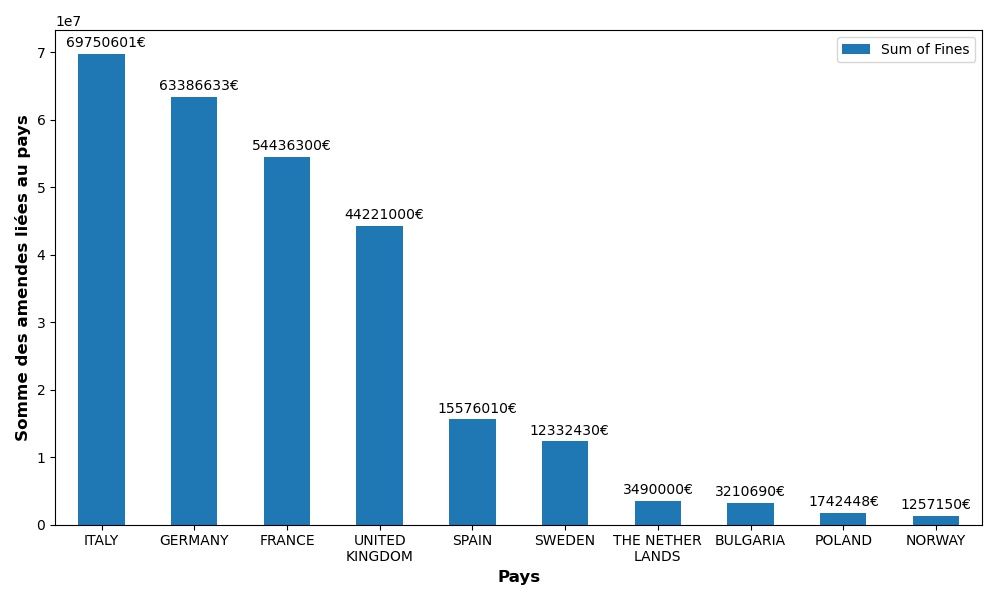
\includegraphics[width=0.7\linewidth]{graphs/top10_countries_fines}
	\caption{Top 10 EU Countries with the highest sum of fines}
 \end{figure}


\newpage

	\begin{multicols}{2}
	\begin{figure}
		[H]\centering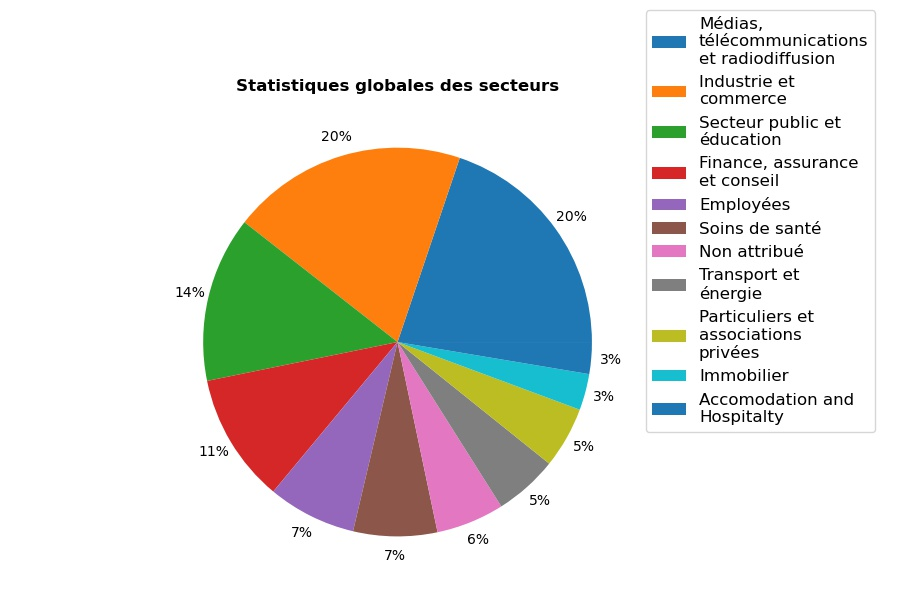
\includegraphics[width=1.0\linewidth]{graphs/sector_data}
		\caption{Top 10 Sectors on piechart with the highest number of fines}
	\end{figure}
	\begin{figure}
		[H]\centering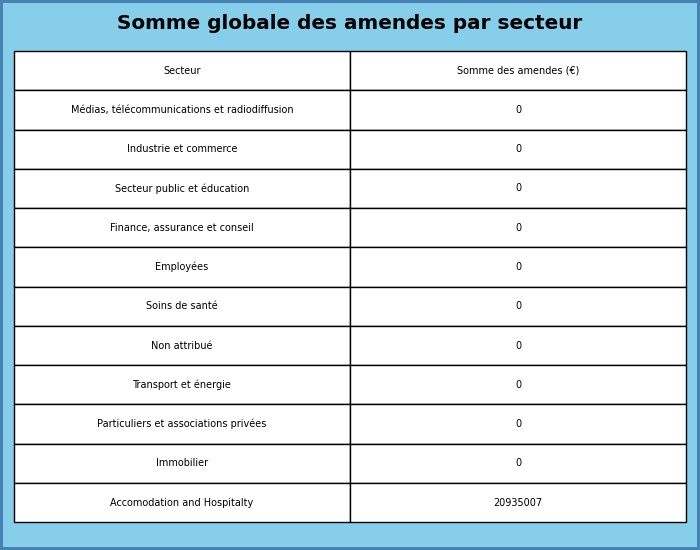
\includegraphics[width=1\linewidth]{graphs/sector_data_fines}
		\caption{Top 10 Sectors with the highest amount of fines}
	 \end{figure}
	
	\end{multicols}
	
	
	
	\begin{figure}
		[H]\centering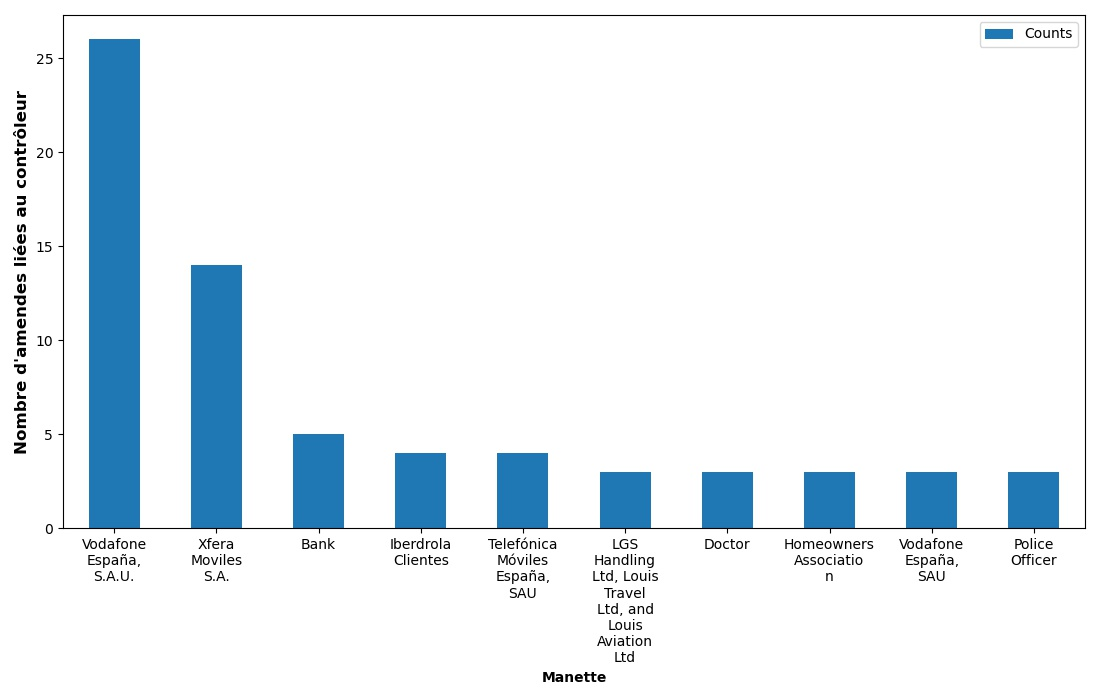
\includegraphics[width=0.6\linewidth]{graphs/top10_controller}
		\caption{Top 10 Companies with the highest number of fines}
	\end{figure}
	
	\begin{figure}
		[H]\centering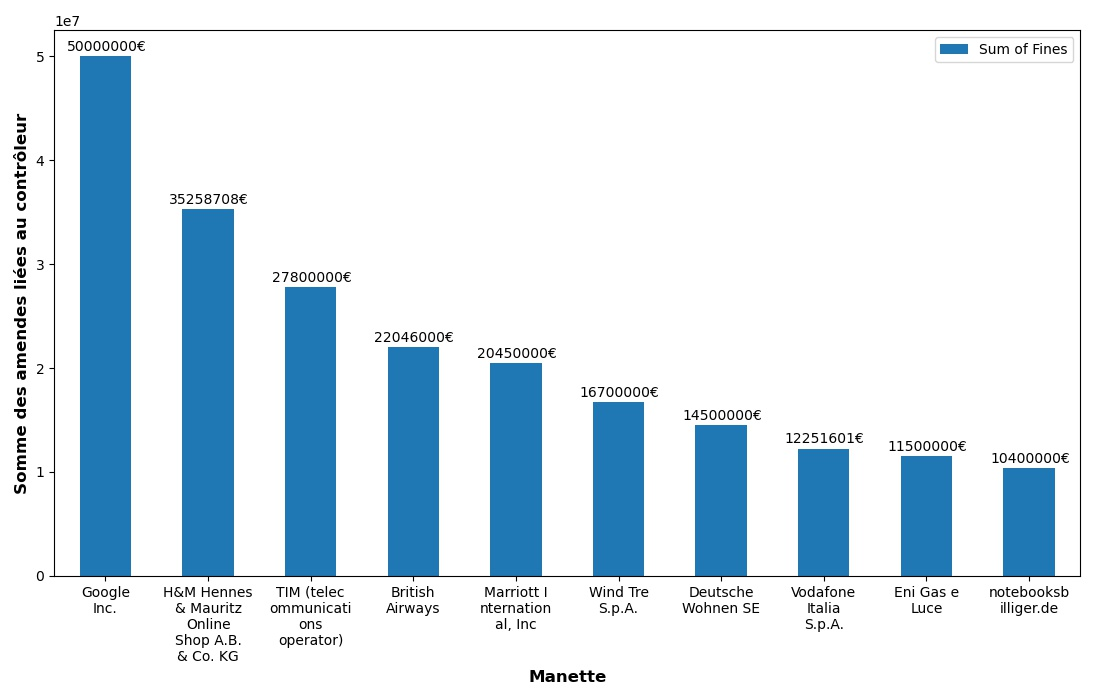
\includegraphics[width=0.6\linewidth]{graphs/top10_controller_fines}
		\caption{Top 10 Companies with the highest amount of fines}
	 \end{figure}



\newpage


	\begin{multicols}{2}
	\begin{figure}
		[H]\centering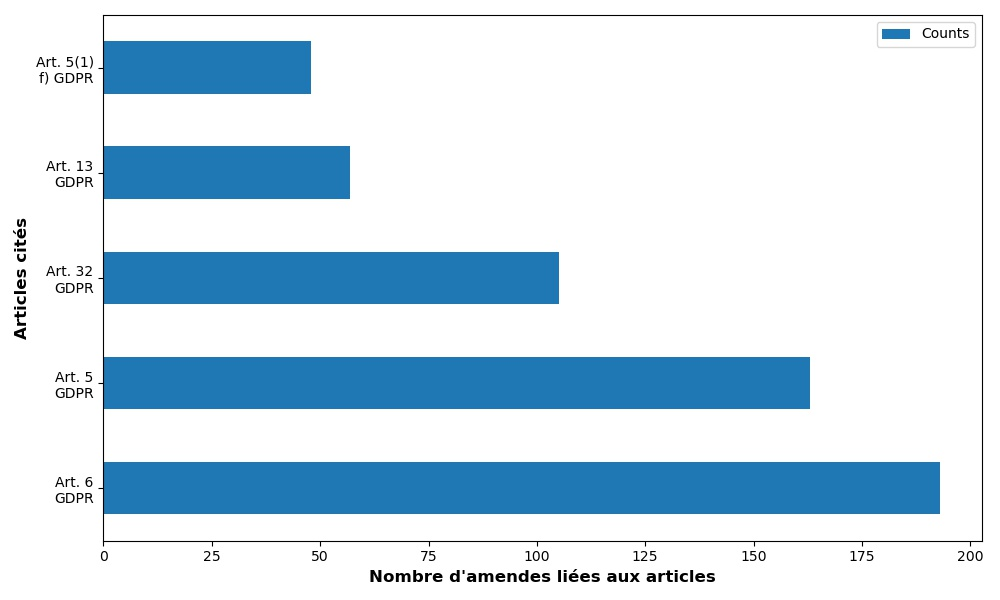
\includegraphics[width=1\linewidth]{graphs/top10_quoted} 
		\caption{Top 5 Quoted Articles with the highest number of fines}
	\end{figure}
	\begin{figure}
		[H]\centering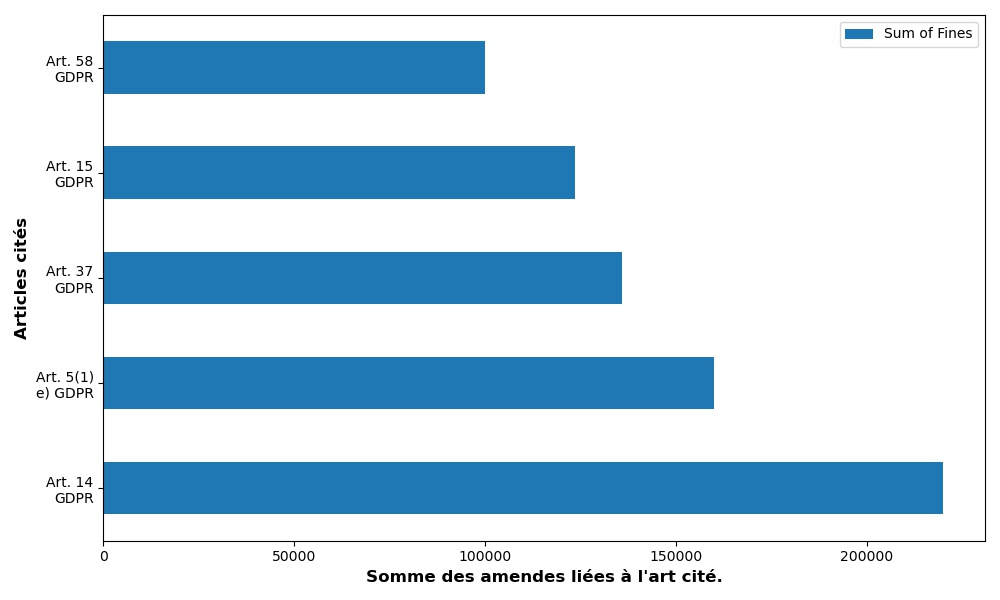
\includegraphics[width=1\linewidth]{graphs/top10_quoted_fines} 
		\caption{Top 5  Quoted Articles with the highest amount of fines}
	\end{figure}
	\end{multicols}
	
	
	\NewsItem{\raggedright{\LARGE Analysis on GDPR enforcement over years}}
	\begin{figure}
		[H]\centering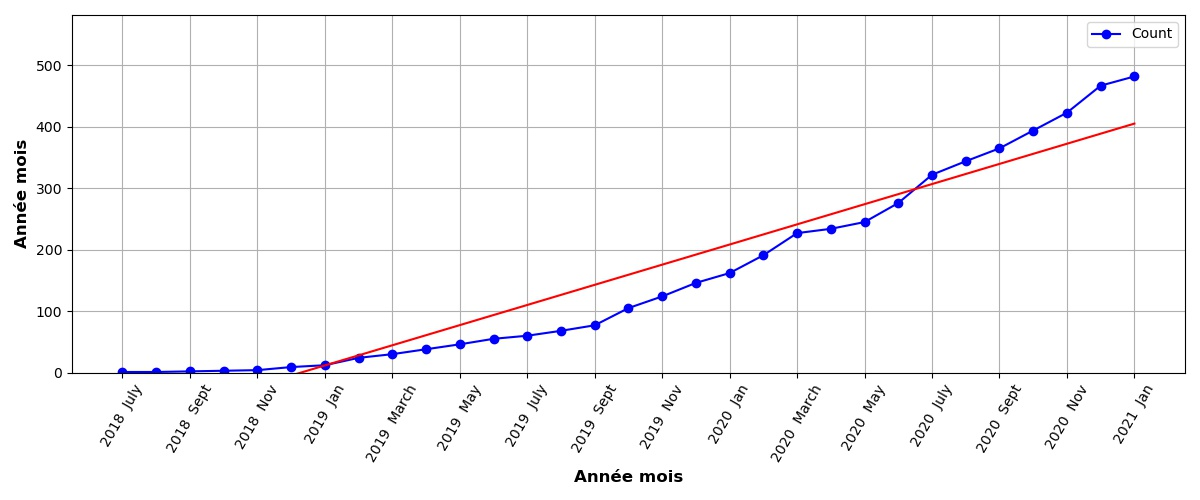
\includegraphics[width=0.8\linewidth]{graphs/acc_nb_cases_graph}
		\caption{Overall Number of Fines (cumulative) }
	\end{figure}
	
	\begin{multicols}{2}
	\begin{figure}
		[H]\centering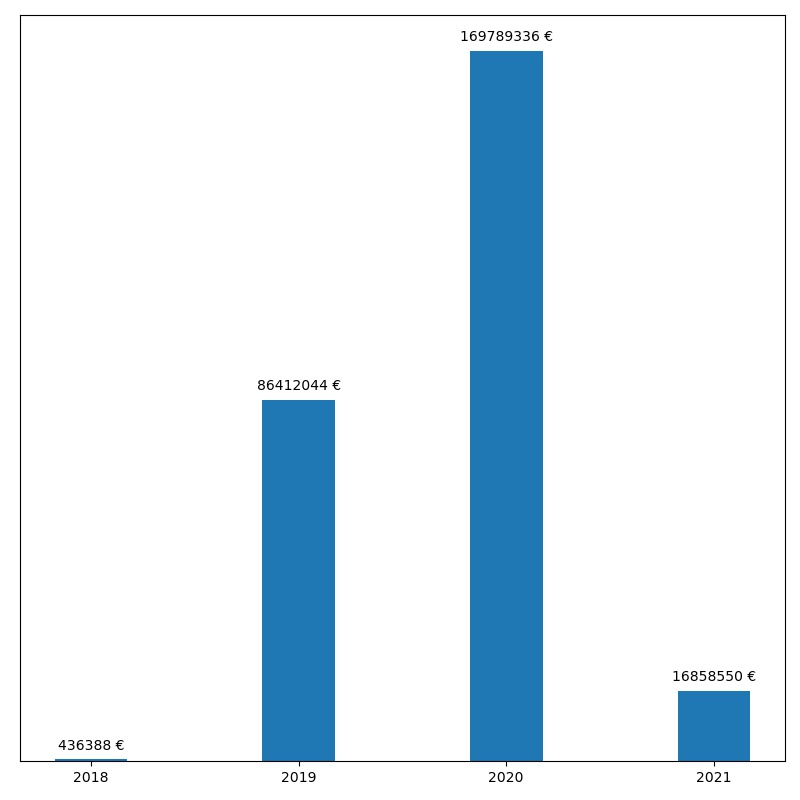
\includegraphics[width=1.0\linewidth]{graphs/SumOfFinesperYear}
		\caption{Overall Amount of Fines per year }
	 \end{figure}
\justify
	GDPR enforcement has accelerated since the first few years, both on the number of enforcement cases as well as the sum of fines. Public awareness and media coverage on privacy and data protection have increased over the years too. However, GDPR is at the risk of failing. According to a research from Brave, this is due to the Data Protection Authorities(DPA) not giving enough human and financial resources to perform their tasks. Only 6 national DPAs have more than 10 specialist tech investigation staff. Half of all national DPAs receive small (€5 million or less) annual budgets from their governments.
	\end{multicols}



\newpage



%Particular Year Statistic
\NewsItem{\raggedright{\LARGE GDPR fines overview in 2020}}

	\begin{multicols}{2}
	
	In 2020, there have been \textbf{321} fines.
	The cumulative total of data protection fines for 2020 now stands at \textbf{169 789 336€}.
	
	\begin{figure}[H]
	\centering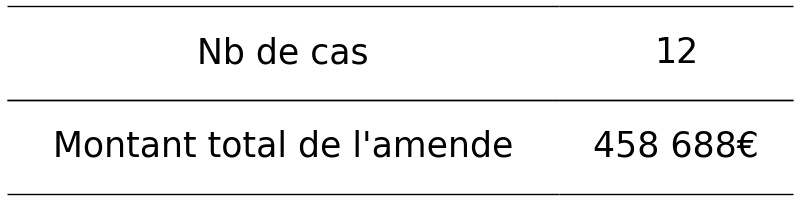
\includegraphics[width=1\linewidth]{graphs/counter_year}
	\end{figure}


	The GPDR fines for 2020 break down for each months as follow :

	\begin{figure}
	[H]\centering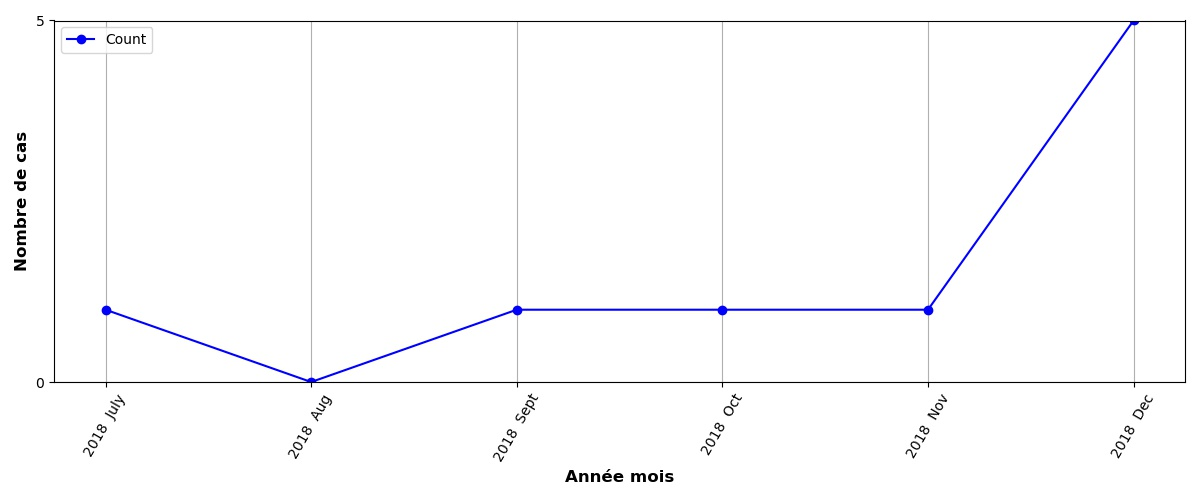
\includegraphics[width = 1.2\linewidth]{graphs/NbFinesPerMonth_year_graph}
	\caption{Small Overview over months in 2020}
	\end{figure}

	\end{multicols}


	\begin{figure}
		[H]\centering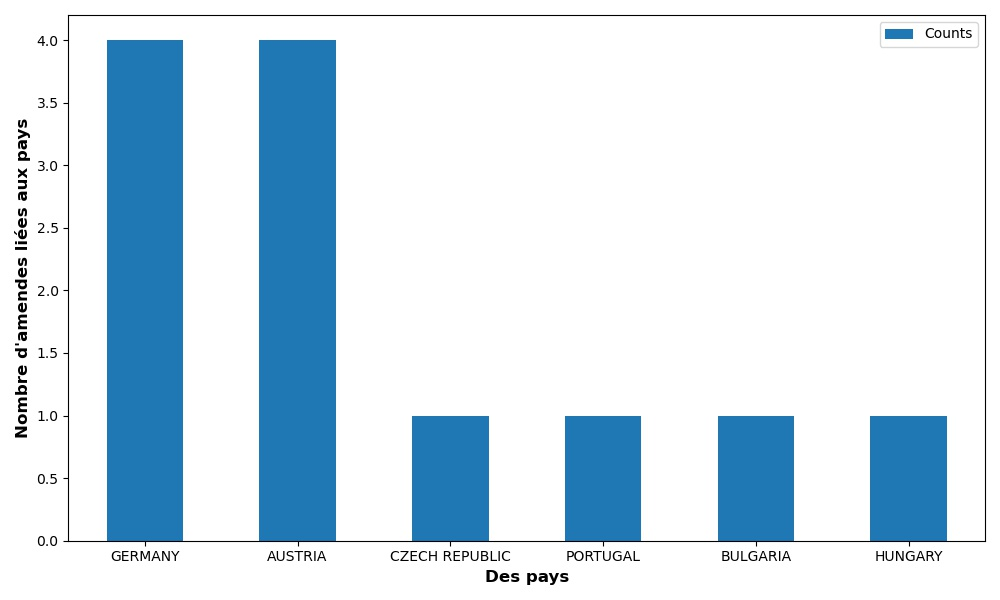
\includegraphics[scale=.5]{graphs/top10_countries_year}
		\caption{Top 10 EU Countries with the highest number of fines in 2020}
	\end{figure}
	\begin{figure}
		[H]\centering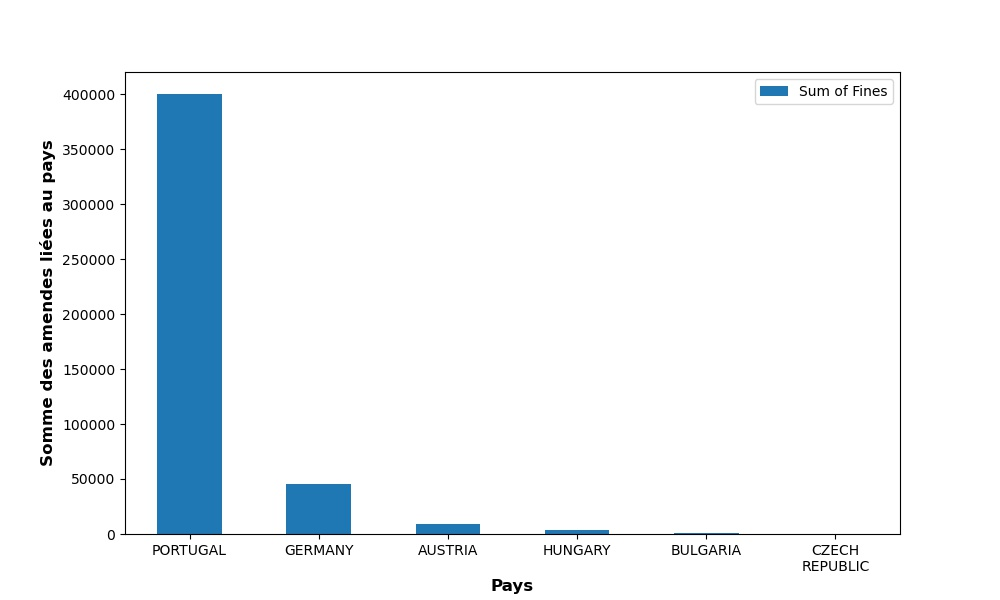
\includegraphics[scale=.5]{graphs/top10_countries_year_fines}
		\caption{Top 10 EU Countries with the highest sum of fines in 2020}
	\end{figure}

\newpage
\justify
	\begin{multicols}{2}
	\heading{3 most recent fines in 2020}{3 pt}
		\begin{itemize}
			\item \textbf{2020-12-30} \newline
			3,000€ fine issued in ROMANIA to ING Bank N.V. Amsterdam - Bucharest office.
			\newline
			The Romanian DPA (ANSPDCP) fined ING Bank N.V. Amsterdam - Bucharest office in the amount of EUR 3,000. The bank had contacted the data subject by e-mail for the purpose of updating his data. At that time, however, the data subject had already terminated his account with the bank, so that the contractual relationship had been terminated. As a result, the data controller had unlawfully processed personal data of the former customer without his consent such as the e-mail address and the name and of the data subject.
			\newline
			\href{https://www.dataprotection.ro/?page=Comunicat_presa_30_12_2020&lang=ro}{More Info}
			\vspace{1cm}
	
			\item \textbf{2020-12-29} \newline
			1,000€ fine issued in ROMANIA to Qualitance QBS SA.
			\newline
			The Romanian DPA (ANSPDCP) fined Qualitance QBS SA EUR 1,000 for a violation of Art. 32 GDPR. The company had sent information by email to 295 individuals, disclosing the email addresses of the other recipients. The ANSPDCP noted that the company had not taken sufficient security measures to ensure the confidentiality of the personal data of the data subjects.
			\newline
			\href{https://www.dataprotection.ro/?page=Comunicat_Presa_29_12_2020&lang=ro}{More Info}
			\vspace{1cm}
	
			\item \textbf{2020-12-28} \newline 18,930€ fine issued in POLAND to Towarzystwo Ubezpieczeń i Reasekuracji WARTA S.A.
			\newline
			The Polish DPA (UODO) fined Towarzystwo Ubezpieczeń i Reasekuracji WARTA S.A. EUR 18,930 for a breach of Art. 33 (1) GDPR and Art. 34 (1) GDPR. In May 2020, the DPA received a notification from a third party about a personal data breach involving an insurance agent acting as a processing agent for Towarzystwo Ubezpieczeń i Reasekuracji WARTA S.A. who sent an insurance policy to an unauthorized addressee by email. The document contained personal data concerning, among others, surnames, first names, residential addresses and information on the subject of the insurance policy. As a result, the supervisory authority asked the controller to clarify whether, regarding the sending of the electronic correspondence to an unauthorized addressee, a risk analysis on the data security of natural persons had been carried out, which is necessary to evaluate whether a data breach had occurred. Such a breach requires notification to the DPA and the individuals affected by the breach. In the letter, the supervisory authority advised the controller how to notify the breach and asked for explanations.Despite the letter requesting explanations, the controller did not report the data breach nor did it inform the data subjects about the incident. The DPA therefore initiated administrative proceedings. Only as a result of the initiation of the procedure did the controller report the personal data breach and inform two individuals affected by the breach.
			\newline
			\href{https://uodo.gov.pl/decyzje/DKN.5131.5.2020}{More Info}
		\end{itemize}
	\end{multicols}

\newpage
\justify
	\begin{multicols}{2}
	\raggedright\heading{Notable fines in 2020}{3 pt}
		\begin{itemize}
			\item The \textbf{largest} fine of 2020 - \textbf{35258708 €} - was issued in GERMANY to Hu0026M Hennes u0026 Mauritz Online Shop A.B. u0026 Co. KG.
			\newline
			\textbf{Summary} : The fashion company with seat in Hamburg operates a service center in Nuremberg. Here, according to the findings of the Hamburg data protection officer, since at least 2014 private life circumstances of some of the employees have been comprehensively recorded and this information stored on a network drive. For example, the company conducted a Welcome Back Talk after employees returned to work after vacation or illness. The information that became known in this context - including information on the symptoms of illness and diagnoses of the employees - was recorded and stored. In addition, according to the Hamburg data protection authority, some supervisors also used the Flurfunk [meaning to hear something through the grapevine) to acquire a broad knowledge of individual employees, for example about family problems and religious beliefs. The information stored on the network drive was accessible to up to 50 managers of the company and was used, among other things, to evaluate the work performance of the employees and to make employment decisions.The data collection became known due to a technical configuration error in October 2019, according to which the data stored on the network drive was accessible company-wide for several hours. After the violation became known, the management apologized to the employees and offered monetary compensation. In addition, also further protective measures were introduced together with the data protection authority. [Note: Concrete legal basis of the fine not yet published - we assume this will mainly be Art. 5 and 6 GDPR)
			\newline
			\href{https://datenschutz-hamburg.de/pressemitteilungen/2020/10/2020-10-01-h-m-verfahren}{More info}
			\vspace{1cm}
		
			\item The \textbf{lowest} fine of 2020 - \textbf{28 €} - was issued in  to Google Ireland Ltd..
			\newline
			\textbf{Summary} : Failure to respond to a data subjects request to access information (Art. 15 GDPR - here: about data processed in the context of Google AdWords) in due time.
			\newline
			\href{https://www.naih.hu/files/NAIH-2020-5553-hatarozat.pdf}{More info}
		\end{itemize}
	\end{multicols}


\newpage

	
	\begin{multicols}{2}
	\begin{figure}
		[H]\centering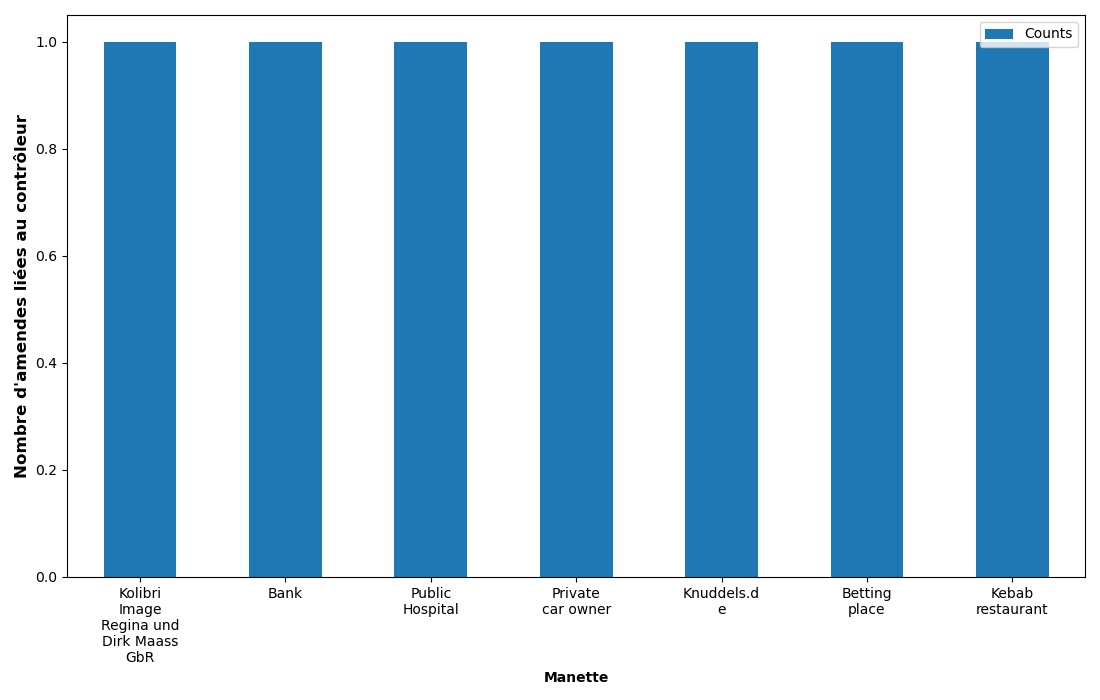
\includegraphics[width=1.0\linewidth]{graphs/top10_controller_year}
		\caption{Top 10 Companies with the highest number of fines in 2020}
	\end{figure}
	\begin{figure}
		[H]\centering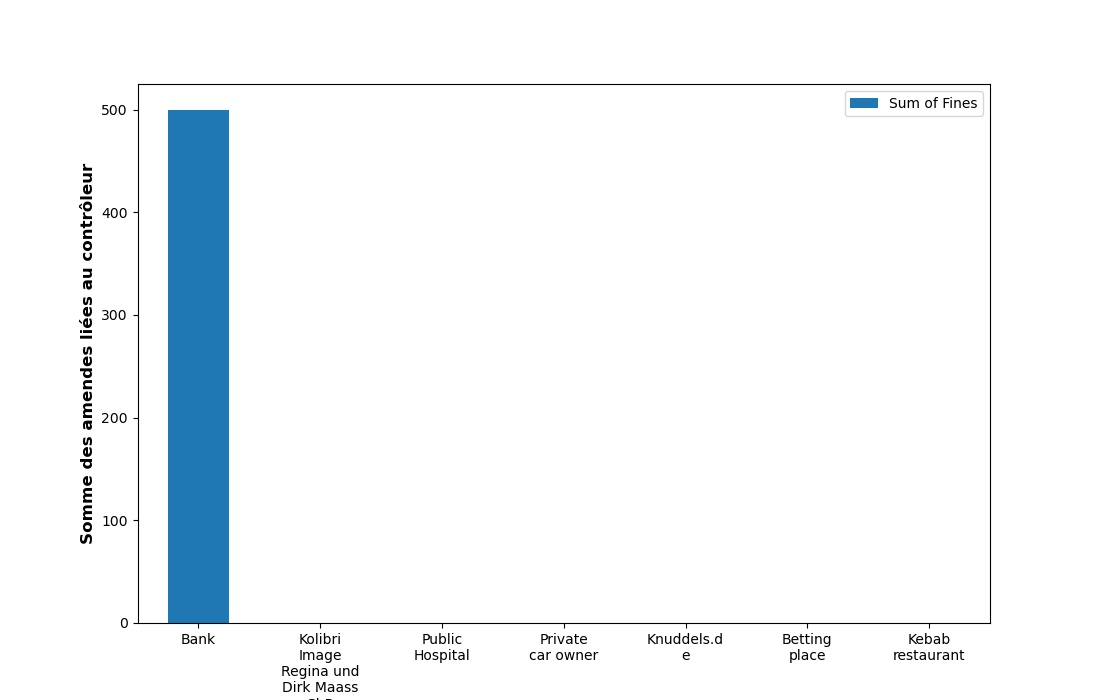
\includegraphics[width=1\linewidth]{graphs/top10_controller_year_fines}
		\caption{Top 10 Companies with the highest  amount of fines in 2020}
	 \end{figure}
	
	\end{multicols}


		
	\begin{multicols}{2}
	\begin{figure}
		[H]\centering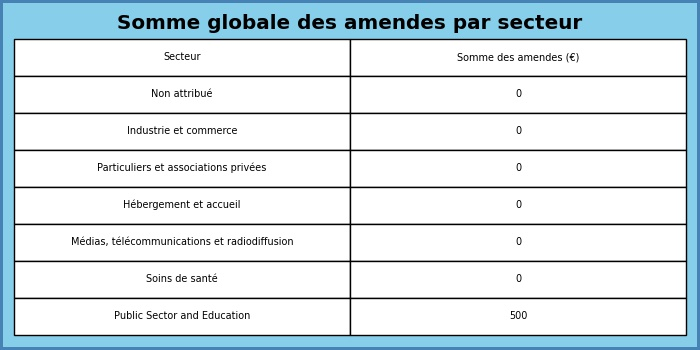
\includegraphics[width=1.0\linewidth]{graphs/sector_data_year_fines}
		\caption{Top 10 Sectors on piechart with the highest number of fines in 2020}
	\end{figure}
	\begin{figure}
		[H]\centering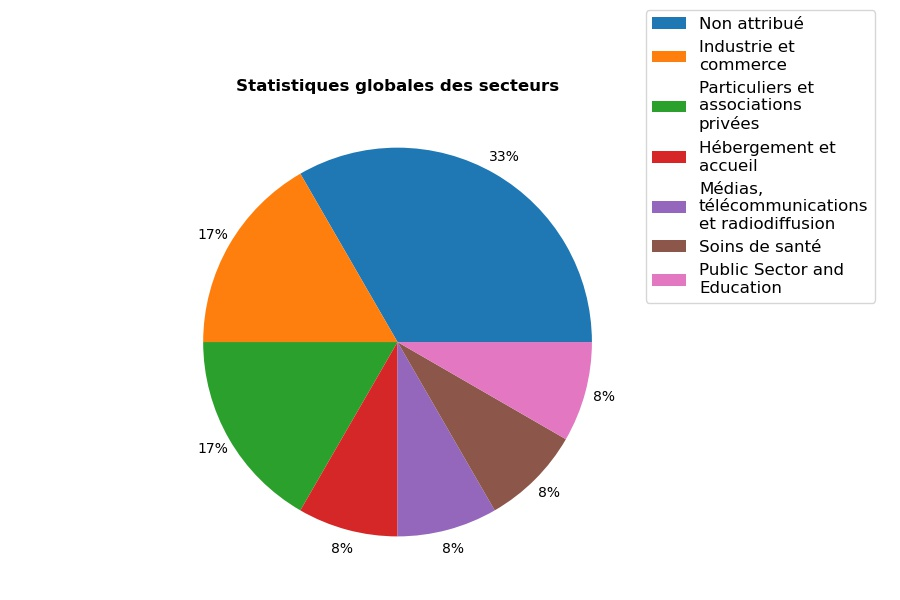
\includegraphics[width=1\linewidth]{graphs/sector_data_year}
		\caption{Top 10 Sectors with the highest amount of fines in 2020}
	 \end{figure}
	
	\end{multicols}

	\begin{multicols}{2}
	\begin{figure}
		[H]\centering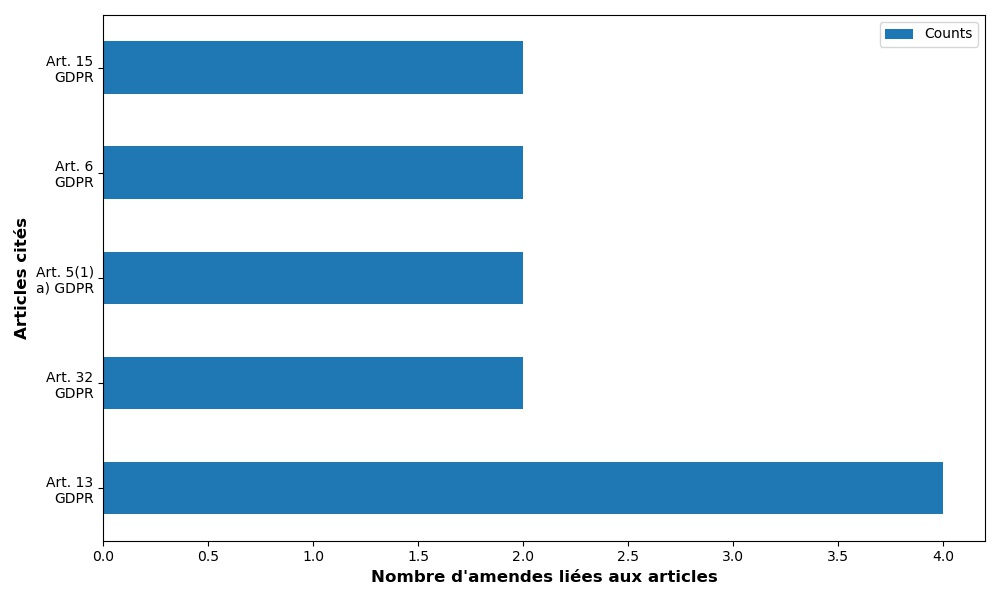
\includegraphics[width=1.0\linewidth]{graphs/top10_quoted_year}
		\caption{Top 10 Quoted Article with the highest number of fines in 2020}
	\end{figure}
	\begin{figure}
		[H]\centering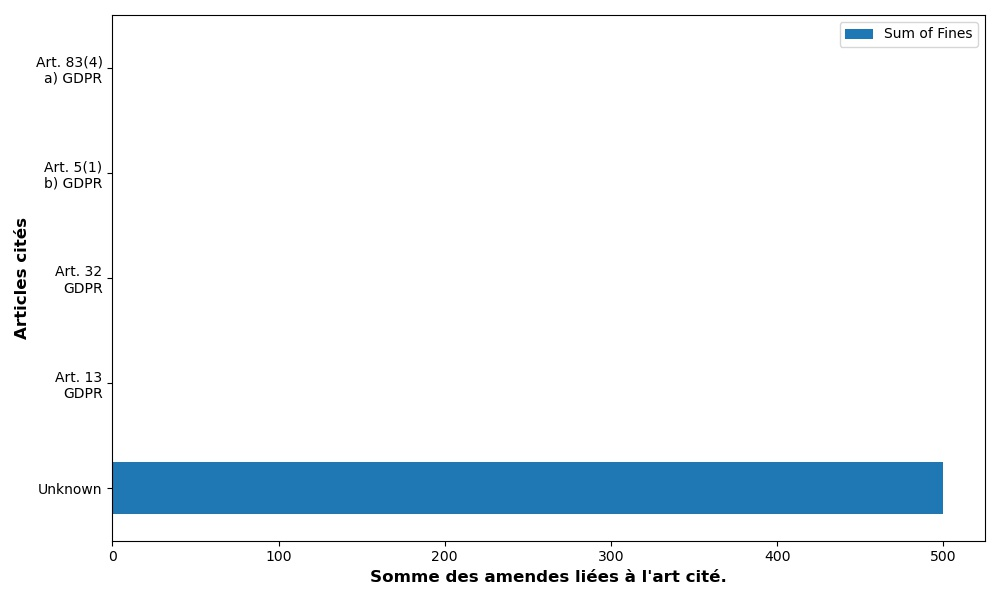
\includegraphics[width=1\linewidth]{graphs/top10_quoted_year_fines}
		\caption{Top 10 Quoted Article with the highest amount of fines in 2020}
	 \end{figure}
	
	\end{multicols}









\vspace*{\fill}
\textbf{References:}\\
\href{https://www.enforcementtracker.com}{https://www.enforcementtracker.com}\\
\href{https://brave.com/wp-content/uploads/2020/04/Brave-2020-DPA-Report.pdf}{https://brave.com/wp-content/uploads/2020/04/Brave-2020-DPA-Report.pdf}\\
\href{https://arxiv.org/pdf/2011.00946.pdf}{https://arxiv.org/pdf/2011.00946.pdf}


\end{document}